\documentclass[a4paper,10pt]{article}

\usepackage[ansinew]{inputenc}
\usepackage[spanish]{babel}
\usepackage{graphicx}
\usepackage{listings}
\usepackage{appendix}
\usepackage{pdfpages}
\usepackage{fancyhdr}
\pagestyle{fancy}

\begin{document}

\lhead{\fancyplain{}{Organizaci\'on de computadoras 66.20 - Turno Martes}}
\rhead{\fancyplain{}{Trabajo Pr\'actico 1}}

\setcounter{page}{2}

\newpage
\thispagestyle{empty}
\tableofcontents

\newpage
\section{Introducci\'on}
  TODO

\section{Resoluci\'on del problema}

  \subsection{unix2dos}
    \subsubsection{Stack frame}
      \begin{center}
	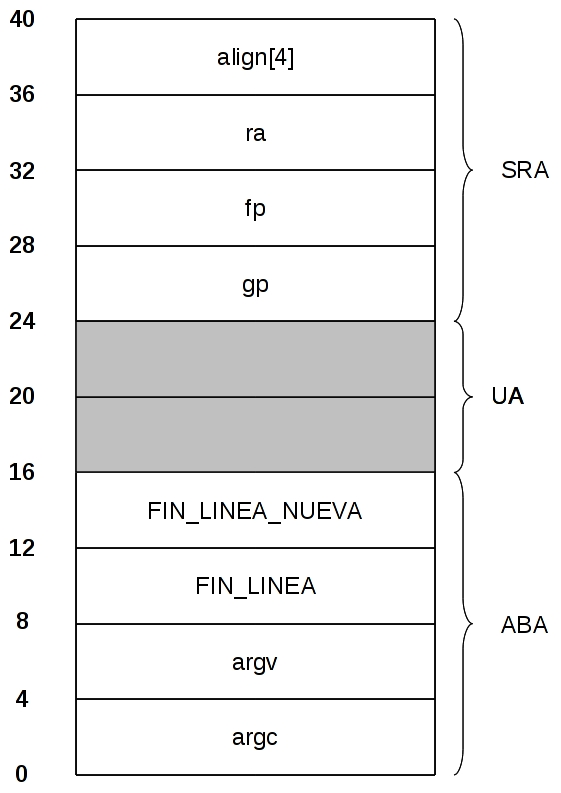
\includegraphics[width=10cm, height=15cm]{DibujosStackFrame/stack-unix2dos(main).jpg}
      \end{center}

 
\section{Preparando el ambiente para NetBSD}
 
\section{Compilando en NetBSD}

\section{Ejecutando los programas en NetBSD}

\section{Casos de prueba}

\newpage
\section{Conclusiones}

%APENDICES
\appendix
\newpage
\section{C\'odigo Fuente}
%  \subsection{unix2dos.S}
%    \lstset{numbers=left, frame=single, breaklines=true}
%    \lstinputlisting{../Codigo/unix2dos.c}
%  \subsection{dos2unix.S}
%    \lstset{numbers=left, frame=single, breaklines=true}
%    \lstinputlisting{../Codigo/dos2unix.c}
%  \subsection{conversor.c}
%    \lstset{numbers=left, frame=single, breaklines=true}
%    \lstinputlisting{../Codigo/conversor.c}

\newpage
\section{Enunciado}
%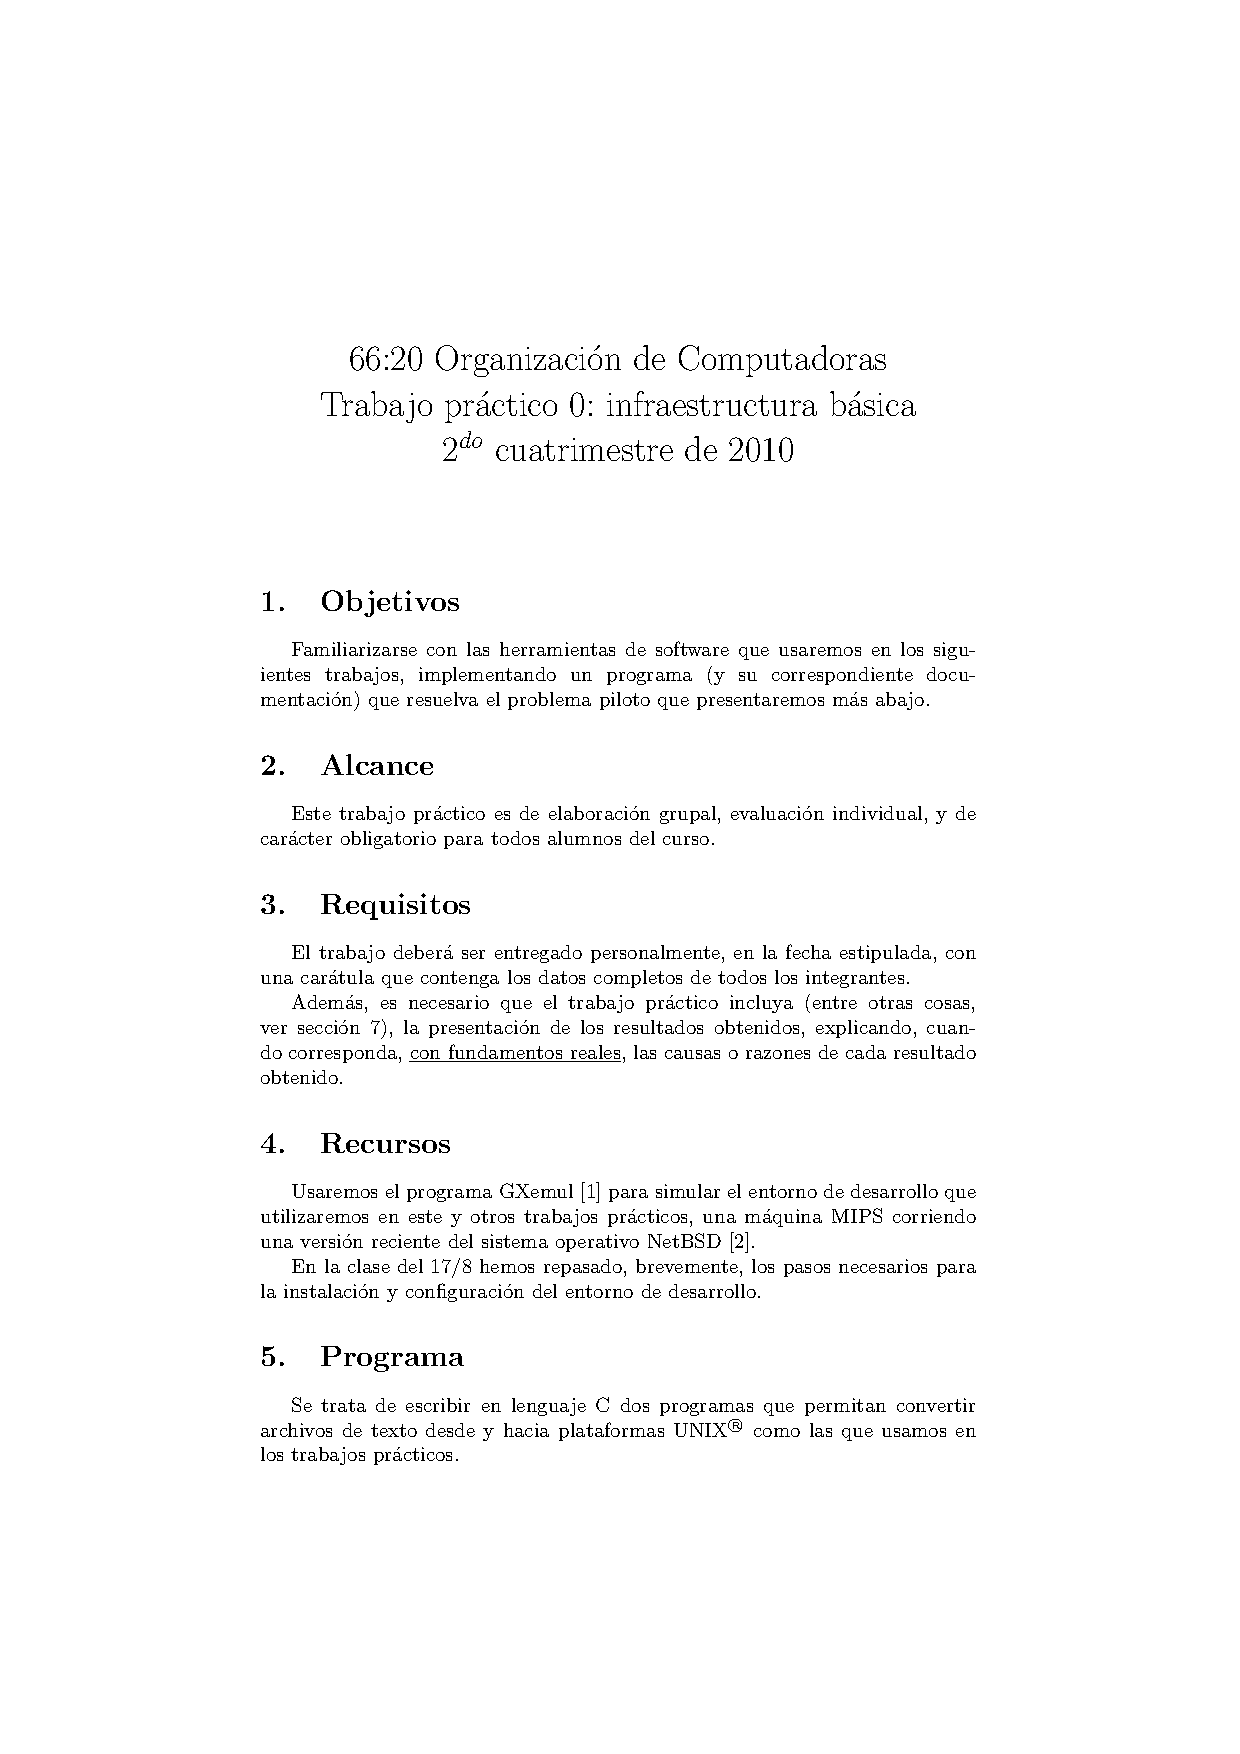
\includepdf[pages=1-3, scale=0.9, pagecommand={\thispagestyle{plain}}]{../tp0-2010-2q.pdf}

\end{document}
